\documentclass[review]{elsarticle}
%%\usepackage[utf8]{inputenc}
%%\usepackage[LGR,T1]{fontenc}
%%\usepackage{graphicx,amsmath}
%%\usepackage[british]{babel}
%%\usepackage[latin9]{inputenc}%SOME KIND OF CLASH WITH THIS ONE
%%\usepackage{array}
%%\usepackage{rotfloat}
%%\usepackage{textcomp}
%%\usepackage{amssymb}
\usepackage{amsmath} 
%% to align equations \usepackage{mathrsfs} % curly font in math, called using mathscr
\usepackage{graphicx}
%%\usepackage{subcaption} % to have two images under one caption
%%\usepackage{subscript}
%%\usepackage{gensymb} %for degree symbol
\setlength{\marginparwidth}{4cm} % to set the width of the marginpar
\usepackage{todonotes}
%%\usepackage{xargs}                      % Use more than one optional parameter in a new commands
%%\renewcommand{\baselinestretch}{1.5}
\bibliographystyle{elsarticle-num}
\begin{document}
\begin{frontmatter}
\title{Advanced novel characterisation of nuclear graphite microstructure via quasi-Bayesian modelling of Scanning Electron Microscopy, N$_2$ adsorption and Hg porosimetry}
\author[plym]{Bradley Moresby-White}
\author[plym]{Katie L. Jones\corref{cor1}}
\ead{katie.jones@plymouth.ac.uk}
\author[plym]{G. Peter Matthews}
\author[plym]{Giuliano M. Laudone}
\cortext[cor1]{Corresponding author.}
\address[plym]{Faculty of Science and Engineering, University of Plymouth, Plymouth, UK}
\begin{abstract}
Nuclear grade graphite is a critical component of those Generation IV reactors
which are graphite-moderated. Reliable characterisation of its microporous
network is crucial for safe and optimal performance. The microstructure, in
particular porosity, dictates material properties and the evolution of those
properties under operational conditions (i.e., oxidation rates, gas diffusion,
and thermal degradation). This project develops and initially validates a
methodology for characterising the surface porosity of IG-110 and IG-430 nuclear
graphites via computational analysis of composite Scanning Electron Microscopy
(SEM) micrographs, covering an FOV (Field of View) comparable with previous
Optical Microscopy (OM) -based works (mm\(^2\) scale). Initial integration of
surface porosity data into a new version of the PoreXpert void network and pore
fluid simulation framework, integrated with Hg porosimetry and N$_2$ adsorption,
produced physically plausible preliminary models of the pore network and
simulated pore-fluid flow properties such as tortuosity, diffusivity, and
permeability. This enhanced characterisation method forms a further useful
methodology in refining models of graphite behaviour, ultimately contributing to
the safe and optimal operation of current and proposed graphite-moderated
nuclear reactors.
\end{abstract}
\begin{keyword}keyword\sep keyword\sep keyword\end{keyword}
\end{frontmatter}

\section{Introduction}
Graphite, a carbon allotrope, is employed as a moderator, neutron reflector and
structural component in Generation IV reactors \citep{MARSDENgeniv}. Nuclear
grade graphite is engineered for this specific use case, characterised by
exceptionally low boron content, high structural strength, thermal stability,
and a high scattering and low absorbent neutron cross-section
\citep{Marsden2016}. 

The internal microstructure of nuclear grade graphite plays a key role in its
mechanical and thermo-physical properties, as well the evolution of these
properties under irradiation \citep{MARSDENgeniv}. Porosity, the proportion of
total volume represented by void space,  is the defining feature of the
microstructure of nuclear-grade graphite.  Porosity differs between grades of
nuclear grade graphite, as a consequence of varying manufacturing processes and
inputs\citep{ARREGUIMENA2022112047}. Key performance and safety-related
phenomena, such as oxidation, gas release and thermal degradation, are modulated
by porosity. Oxidation rates are typically higher where open porosity is
distributed uniformly, as the ease with which closed pore surface area can be
incrementally accessed increases \citep{PAUL2022132}. Porosity also modulates
gas diffusion, with a sufficiently strong correlation coefficient to enable the
estimation of the effective diffusion coefficient from total porosity alone
\citep{KANE2018369}. Diffusion rate then influences the rate of degradation,
determining whether the behaviour under oxidative conditions will be
diffusion-controlled or kinetic-controlled \citep{MATTHEWS2021111245}. 

\subsection{Indirect and Direct Characterisation of Porosity}

Among the primary experimental techniques for the indirect characterisation of
porosity are Mercury (Hg) intrusion porosimetry, Helium (He) pycnometry, and
Nitrogen (N$_2$) adsorption \citep{ARREGUIMENA2022112047, JONES2020256HgHe,
CONTESCU2019663}. No individual experimental technique is capable of
characterising the pore size distribution. 

The limitations  of these techniques increase the attractiveness of direct
characterisation methods, where the pores themselves are characterised. Previous
studies involved quantifying channel porosity  by optical or electron microscopy
\citep{Huang2014, Huang2019, Kane2011a, Kim2010,
Taylor2016,huang2021statistical, ARREGUIMENA2022112047}. Most of these works
have employed optical microscopy, generating datasets based on thousands of
pores, but operating at a low resolution and objective relative to SEM analysis
\citep{Huang2019, Kane2011a, Taylor2016}. In addition, the low objective
required to image large areas via optical microscopy necessitates pore diameter
thresholds which reach in some cases 50 µm², excluding a significant proportion
of the PSD indicated by experimental methods \citep{Huang2019, Kane2011a,
Taylor2016}. 

An erroneous assumption in some previous studies is the equivalence of channel
porosity and open porosity, leading to significant discrepancies when compared
with manufacturer-supplied open porosity values \cite{Kane2011a}. 

This assumption may be predicated on the rationale that during resin
impregnation, surface analysis techniques will exclusively identify the pore
network through which the resin has percolated, as opposed to the closed pore
volume incidentally exposed by sample preparation. Thus, it is reasoned, surface
porosity is a reliable estimate of total porosity where resin impregnation is
implemented. However, channel porosity is invariably a subset of the total open
porosity. This is a consequence of the fact that pores are larger than the
throats connecting them to the surface, which is the feature classified in
microscopy methods. The result is that where surface analysis is employed, the
full volume of each pore is not represented fully by a micrograph of the
surface.

\todo{For them to disagree with the above they also have to give up on
pore shielding, which would then invalidate their use of Hg porosimetry
to derive a PSD, as it requires pore shielding to cancel out their other
assumption. Nice}

\subsection{Objectives of the Present Study}

The primary objective of this work is to develop and validate a method of
quantifying the surface visible porosity of nuclear-grade graphites via Scanning
Electron Microscopy (SEM) micrographs, to then be integrated into the
multi-technique inverse modelling method of PoreXpert. This method inversely
models to determine the set of parameters that produces a percolation curve
minimally different from the intrusion curve derived from Hg porosimetry and
N$_2$/Kr adsorption, and now also SEM-derived channel porosity. The software
therefore produces a simulated pore network on which calculations can be
performed \citep{MatthewsPoreXpert2025}.


The apparent porosity of the surface, which typically includes channels and
voids very near the surface, provides an entirely new experimental input for The
modelling process outlined above. As porosity is derived not only from surface
pores but also from pores adjacent to them just below the surface, apparent
surface porosity is here referred to as channel porosity rather than surface
porosity. The pores identified by the electron micrograph of the surface  are
approximated as channels running through the sample from each visible
pore-throat \cite{MatthewsPoreXpert2025}. The channel porosity estimate replaces
or complements porosity estimates from Hg porosimetry and/or pycnometry, in
effect replacing indirect characterisation with direct characterisation.


The SEM-derived channel porosity characterisation of this work utilises
composite micrographs, composed of 225 individual micrographs per sample, fused
into a single composite. The general form of this stage is the same as the with
SEM-based characterisation of IG-110  by other workers
\citep{huang2021statistical}. While this approach provides a comparable
analytical area to previous optical microscopy (OM) based studies, it offers a
substantial increase in both resolution and magnification. The subsequent
analysis and following modelling is founded upon tens of thousands of individual
pores per sample, resolved at high definition, from which a channel porosity
percentage and a detailed pore size distribution (PSD) are derived for each
sample. The intrinsically higher resolution afforded by Scanning Electron
Microscopy (SEM) facilitates the significantly lower pore diameter thresholds,
yielding a channel porosity and PSD of enhanced statistical representativeness.

This method therefore intends to construct more representative pore network
models, leading to network characteristic calculations, such as permeability or
diffusivity,  which better represent the physical nature of the samples being
modelled.

The validation of this integrated approach is contingent upon its ability to
generate a full percolation curve—derived from the combination of SEM-derived
channel porosity, mercury (Hg) porosimetry data, and Grand Canonical Monte Carlo
(GCMC) modelled N$_2$ adsorption—that yields an open porosity value in close
agreement with that determined experimentally by Helium (He) pycnometry.

\todo{I say here surface analysis identify throats not pores, then
the distinction I make between this work and others, where the high intensity
threshold leads to the identification of pore throats not pore contours, I think
may need to be thought through.}

\section{Methodology}

\subsection{Materials}

Virgin graphite samples of two grades, IG-110 and IG-430, were supplied by Toyo
Tanso Ltd\texttrademark{}, Osaka, Japan. The properties of both grades are
tabulated (Table ~\ref{tab:materialstable}). IG‑110 is employed in the
three existing HTGRs worldwide, while IG‑430 is designed to deliver increased
density, strength, and thermal conductivity for future
applications \citep{toyotanso_atomic_nuclear}.

\begin{table*}[b]
  \centering
  \caption{Formation characteristics and properties of IG-110 and IG-430 nuclear grade graphites \citep{Jones2018, ARREGUIMENA2022112047}}
  \label{tab:materialstable}
  \resizebox{\columnwidth}{!}{%
    \begin{tabular}{l l c c c c c}
      \hline
      Grade   & Coke source & Bulk density/g cm$^3$ & Filler particle size/$\mu$m & Tensile strength/MPa & Young's modulus/GPa & Thermal conductivity/W m$^{-1}$K$^{-1}$\\
      \hline
      IG‑110  & Petrol          & 1.77                  & 10                           & 25                     & 9.8                   & 120 \\
      IG‑430  & Pitch             & 1.82                  & 10                           & 37                     & 10.8                  & 140 \\
      \hline
    \end{tabular}%
  }
\end{table*}

\subsection{Sample preparation}
Cuboids were subsampled from virgin graphite blocks, with dimensions of
approximately 10 mm x 10 mm x 100 mm. The subsamples were further subsampled
into cuboids of side lengths 7 mm, providing 3 cuboids per grade. Samples were
polished via SiC polishing pads up to a grit size of P5000, to minimise
topographical variations induced by sample preparation that may cause artefacts
during SEM imaging or low pressure gas adsorption \citep{Fang2022,Jones2018}.
Samples were sonicated in 2-propanol for 24 h to remove silica particles
introduced during polishing, then dried under vacuum for 12 h at $305 \pm 5
\,^\circ\mathrm{C}$ using the BELPREP-vac (MicrotracBEL, Japan) to remove residual
2-propanol.

\subsection{Scanning Electron Microscopy (SEM)}

The JEOL IT510 Scanning Electron Microscope was employed to generate the
contiguous set of micrographs from which the full composite micrograph is
assembled. The Image Montage capability within the JEOLInScope package performed
this function, capturing multiple micrographs via a motorized stage, moving the
electron beam over the specified area with a set overlap for each consecutive
micrograph. Applied parameters are tabulated (Table
~\ref{tab:microscopy_parameters}). Stigmation, contrast, and brightness were
automatically adjusted, with analysis of the metadata for all 1,350 micrographs
demonstrating that shifts in contrast and brightness were insignificant, with no
impact on the selection of the intensity threshold for the full composite (Table
~\ref{tab:contrast-brightness-summary}). 

\begin{table}
  \centering
  \caption{Summary of the contrast and brightness applied by the automatic adjustment of the SEM software package for all micrographs, expressed as percentages of respective maxima for each sample.}
  \label{tab:contrast-brightness-summary}
  \resizebox{\columnwidth}{!}{%
  \begin{tabular}{lrrrr}
    \hline
    Sample & Avg. Contrast (\%) & Std. Contrast  (\%) & Avg. Brightness (\%) & Std. Brightness (\%) \\
    \hline
    IG-430B & 98.01 & 1.02 & 99.69 & 0.08 \\
    IG-430C & 98.16 & 0.82 & 99.83 & 0.08 \\
    IG-430F & 97.70 & 0.81 & 99.58 & 0.14 \\
    IG-110B & 95.86 & 0.72 & 99.26 & 0.13 \\
    IG-110C & 94.03 & 0.93 & 99.38 & 0.13 \\
    IG-110F & 98.20 & 0.70 & 99.69 & 0.13 \\
    \hline
  \end{tabular}
  }
\end{table}

\begin{table}
  \centering
  \caption{Parameters for composite assembly captured with the JEOL IT510 SEM using Image Montage Mode}
  \label{tab:microscopy_parameters}
  \begin{tabular}{l l}
    \hline
    Parameters & Value \\
    \hline
    Magnification ($\times$)                    & 1000 \\
    Resolution (µm/px)               & 0.1 \\
    Surface area per micrograph (µm²) & 12\,288 \\
    Overlap (\%)                          & 10 \\
    Micrographs per sample (n)            & 225 \\
    \hline
  \end{tabular}%
\end{table}

Each micrograph represents 12,288 µm² of sample surface, with each sample
consisting of 225 micrographs, yielding a total imaging area of 2.765 mm² per
sample. With 3 samples analysed per grade, the total scanned area per graphite
grade is 8.294 mm². 

\subsection{Composite assembly}

Stitching/composite assembly, the assembly of the overlapping micrographs into a
single composite, was performed via an enhanced phase correlation method,
operated as an ImageJ plugin \citep{ Preibisch2009}.The approach optimises
micrograph position globally, is sub-pixel accurate and smooths the transitions
between micrographs by a non-linear intensity blending function.Testing
indicated that adjustment of the blending parameter had no discernable impact on
the final composite micrograph or channel porosity values. Further information
can be found in the Supplementary Information.

The resulting composites exhibit no visible delineation between individual
micrographs, cover an area comparable with previous works, and distinguish
porosity and bulk (Figure \ref{fig:IG430C split scaled}
\citep{Huang2019,Kane2011a,huang2021statistical}). 

	\begin{figure}
		\centering
		\includegraphics[width=0.9\columnwidth]{./Media/C1-IG430c fusion cropped split scaled.jpg}
		\caption{Fully assembled SEM composite: IG-430 Sample C, 1000×  magnification,
     5 kV accelerating voltage. Bar = 250 µm.}
		\label{fig:IG430C split scaled}
	\end{figure} 

\subsection{Computation of Channel Porosity}
\subsubsection{Intensity/Greyscale Thresholding}

For the construction of the histogram of intensity, where porosity is to be
distinguished, per 8-bit micrograph \(E\) (pixel values \(0 \le E(x,y) \le 255\)),
the intensity histogram \(H(i)\) is computed for \(i=0,1,\dots,255\).
\[
H(i) = \sum_{x=1}^{M}\sum_{y=1}^{N} \mathbf{1}\{E(x,y)=i\},
\]
where \(M\) and \(N\) are the micrograph width and height (in pixels), and
\[
\mathbf{1}\{E(x,y)=i\} =
\begin{cases}
1, & \text{if the pixel at }(x,y)\text{ has intensity }i,\\
0, & \text{otherwise.}
\end{cases}
\]

The indicator function \(\mathbf{1}\{E(x,y)=i\}\) increments the bin
corresponding to that greyscale value. The double sum
\(\sum_{x=1}^M\sum_{y=1}^N\) performs  across each pixel in the micrograph
resulting in a histogram \(H(i)\) of 256 bins, each bin representing number of
pixels in the micrograph at each greyscale value \(i\). 

Intensity thresholding, performed on \(H(i)\), determines a greyscale value at
which porosity and bulk (i.e., foreground and background) are distinguished.
Global automatic thresholding algorithms optimise by differing criteria (i.e.
maximisation of inter-class variance, minimisation of intra-class variance) to
determine threshold(s). Thresholding aims to select an greyscale value that
binarises porosity, minimising Type I and II errors, as evaluated by the
operator.

Evaluation of the 17 automatic global intensity thresholding algorithms
available in ImageJ revealed that none were able to distinguish between porosity
and bulk with the sensitivity required to allow the classification of pores for
the given histogram (Figure ~\ref{fig:Try All Thresholding Methods}). In every
case, the histogram \(H(i)\) produced by this method exhibited only a single
peak, yielding no statistically distinct intensity classes (Figure
\ref{fig:histogramnobimodal}). Automatic thresholding selects a threshold
between classes/peaks, consequently, no global intensity thresholding method
could distinguish porosity and bulk in this dataset.

    \begin{figure}
		\centering
    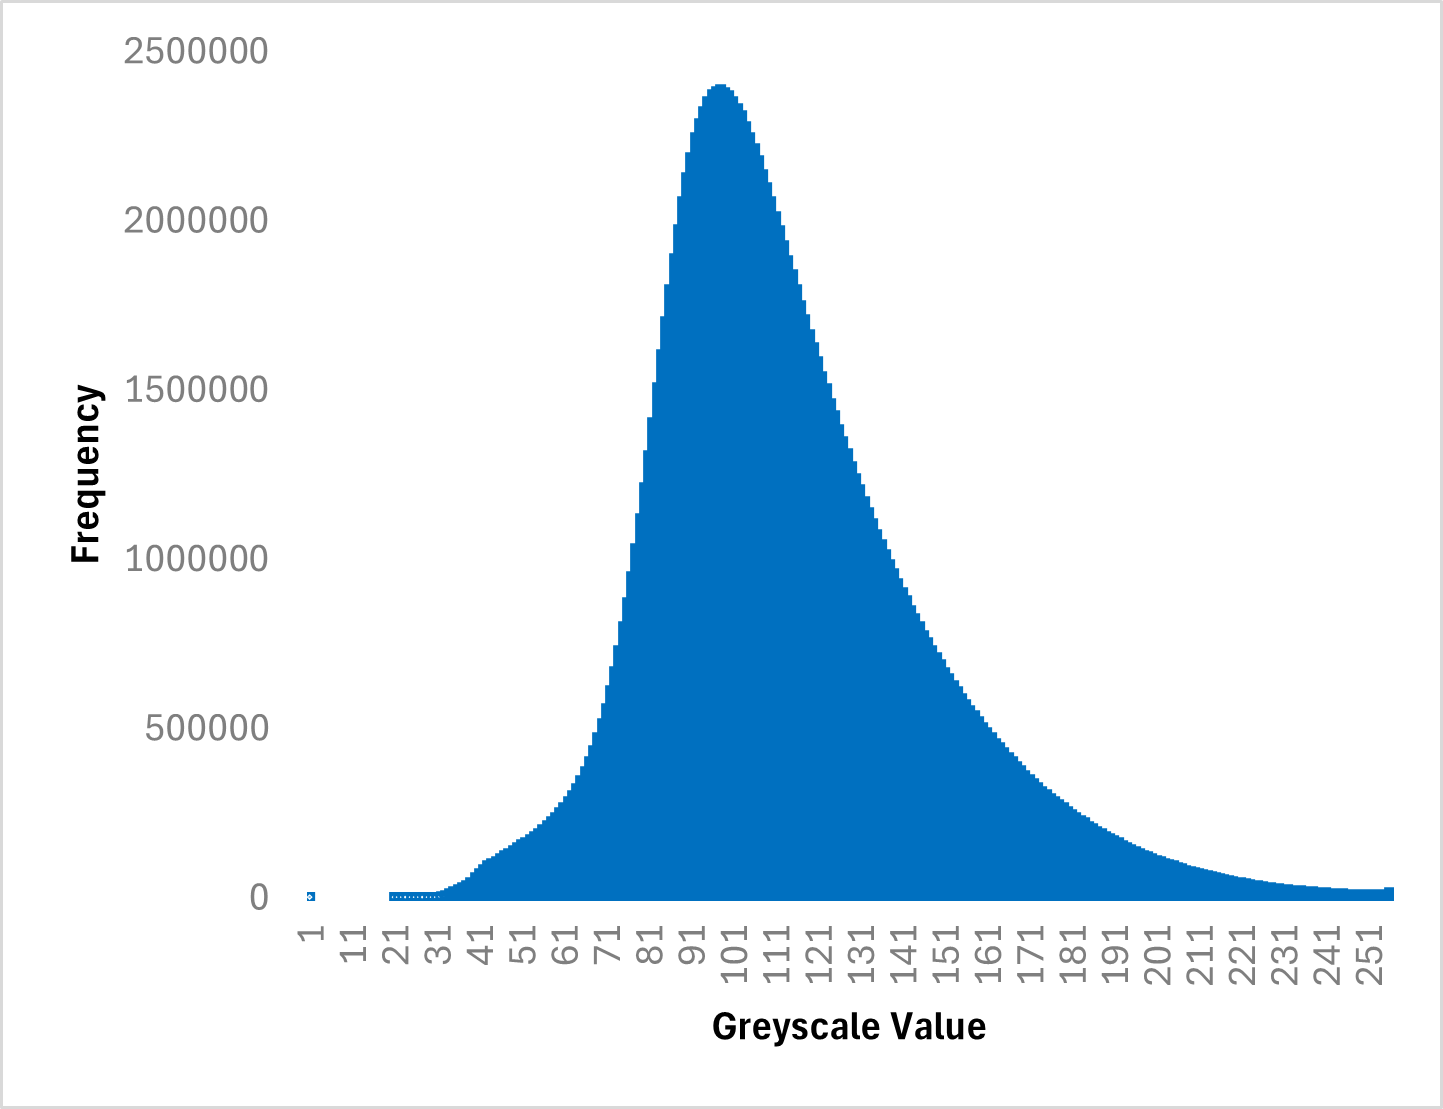
\includegraphics[width=0.9\columnwidth]{./Media/IG430F Greyscale Histogram.png}
		\caption{PLACEHOLDER DRAFT: Histogram of greyscale values for IG-430 Sample F, 1000×, Showing skewness and unimodality}
		\label{fig:histogramnobimodal}
	\end{figure} 

	\begin{figure}[!htbp]
		\centering
		\includegraphics[width=0.9\columnwidth]{./Media/MontageIG430C Methods.jpg}
		\caption{Thresholded Micrograph of IG-430 Sample C at $1000\times$ Magnification. Methods are placed sequentially from right to left, row by row. 
      (a) Default
			(b) Huang
			(c) Huang2
			(d) Intermodes
			(e) IsoData
			(f) Li
			(g) MaxEntropy
			(h) Mean
			(i) MinError(I)
			(j) Minimum
			(k) Moments
			(l) Otsu
			(m) Percentile
			(n) RenyiEntropy
			(o) Shanbhag
			(p) Triangle
			(q) Yen}
		\label{fig:Try All Thresholding Methods}
	\end{figure}  

	A human-in-the-loop (HITL) approach was therefore undertaken (Figure
	~\ref{fig:Final Workflow}). For each sample, the composite was subsampled and
	examined the threshold determined, then applied to the full composite of that
	sample. The intensity thresholds were higher in this work than in previous
	optical microscopy works, at $0.95 \pm 0.075$ normalized between 0-1 over the
	8-bit range of 0-255, capturing the pore throats rather than pore contours.
	\citep{Kane2011a,Huang2019}.


\begin{figure}[!htbp]
    \centering
    \includegraphics[width=0.9\columnwidth]{./Media/Newprocessmodel.png}
    \caption{Full thresholding workflow detailing the process of micrograph generation,
     composite assembly, subsampling, intensity thresholding, and pore diameter thresholding.}
    \label{fig:Final Workflow}
\end{figure}

An output from this process, selected at random, demonstrates the result of the
HITL approach (Figure ~\ref{fig:dualintensitythreshig430f}).

\begin{figure}[!htbp]
    \centering
    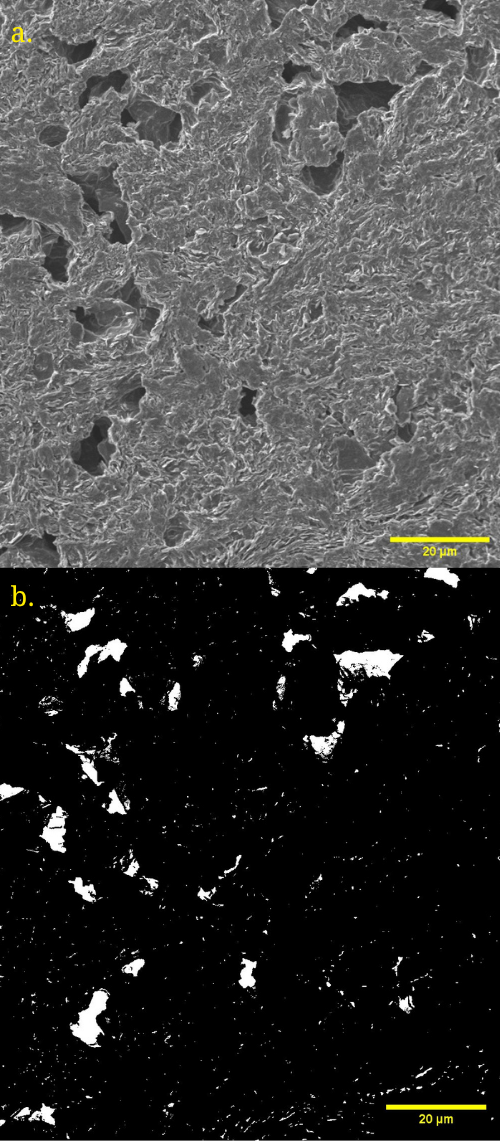
\includegraphics[width=0.9\columnwidth]{./Media/intensitythresholdexampleig430fdual.png}
    \caption{DRAFT: IG430F raw (a) and following intensiy thresholding (b)}
    \label{fig:dualintensitythreshig430f}
\end{figure}

	\subsubsection{Pore Diameter Thresholding}
    
  Pore size thresholds were imposed in this work to restrict the classification
  of pores to a range where binarisation is deemed sufficiently accurate via
  sensitivity analysis \citep{Taylor2016, Huang2019, Kane2011a}. 
      
  Significant changes in the total pore count result from minor alterations to
  the threshold (Table ~\ref{tab:thresholdsandvariationsIG430F}). The
  total area of pores exhibits significantly less variation as a function of
  pore diameter threshold (Table ~\ref{tab:thresholdsandvariationsIG430F}).
  Analysis of the resulting PSDs and sensitivity analysis at each threshold as
  indicated a pore area threshold of 1 µm\(^2\) (diameter = 1.12 µm) was the
  optimal compromise between Type I and II errors (Figure
  ~\ref{fig:improvedporediademo}, Table
  ~\ref{tab:thresholdsandvariationsIG430F}),

   \begin{table}
  \centering
  \caption{Effect of different pore area thresholds on a subsection of IG-430F, showing the resulting pore count, total area, average pore size, and percentage area.}
  \label{tab:thresholdsandvariationsIG430F}
  \resizebox{\columnwidth}{!}{%
    \begin{tabular}{l c c c c c c}
      \hline
      \textbf{Area Threshold} ($\mu$m$^2$) & 0 & 0.5 & 1 & 2 & 4 & 8 \\
      \hline
      Count & 254261 & 11375 & 6 & 4085 & 2812 & 1881 \\
      Total Area (µm²) & 71219 & 56722 & 53361 & 50063.63 & 46518 & 41161\\
      Average Size (µm²) & 0.28 & 4.987 & 8.229 & 12.255 & 16.543 & 21.883 \\
      \% Area & 4.786 & 3.812 & 3.586 & 3.364 & 3.126 & 2.766 \\
      \hline
    \end{tabular}%
  }
\end{table}

\begin{figure}[!htbp]
    \centering
    \includegraphics[width=0.35\columnwidth]{./Media/ImprovedPoreDiaDemo.png}
    \caption{Effect of minimum area threshold on pore identification in subsample of IG-110 Sample B. Highlighted circles denote features which surpassed the previous threshold(s) only, indicated by colour. Thresholds applied (a–f, left-to-right, top-to-bottom): None, 0.5 µm\(^2\), 1 µm\(^2\), 2 µm\(^2\), 4 µm\(^2\), and 8 µm\(^2\).}
    \label{fig:improvedporediademo}
\end{figure}

\subsubsection{Channel Porosity Analysis and Calculation}
Channel porosity was calculated using the “Analyse Particles” function in
ImageJ, identifying pixels surpassing the intensity threshold, generating
connected regions (i.e., pores) via a flood-fill algorithm. Connectivity in the
flood fill algorithm was based on the 8-connected (Moore neighbourhood)
criterion, where a pixel at $(x,y)$ is considered connected to its eight
immediate neighbours:

\begin{multline*}
(x-1,y-1),\; (x-1,y),\; (x-1,y+1),\; (x,y-1),\\[4pt]
(x,y+1),\; (x+1,y-1),\; (x+1,y),\; (x+1,y+1)
\end{multline*}

Any two pixels that exceed the intensity threshold and are either directly
adjacent or diagonally connected are classified as belonging to the same region
(pore). The area and diameter per pore is calculated by converting the pixel
count into physical area (i.e., 10 pixels per micrometre). Regions that do not
meet the area/diameter threshold are omitted. 

Output from intensity thresholding and pore diameter thresholding for the above
parameters is exemplified (Figure ~\ref{fig:C1-ig430f fused cropped 8 bit one
color threshed subsample 2um areathresh}). The final output was both a pore size
distribution (PSD) and channel porosity (\%) per sample.

\begin{figure}[!htbp]
    \centering
    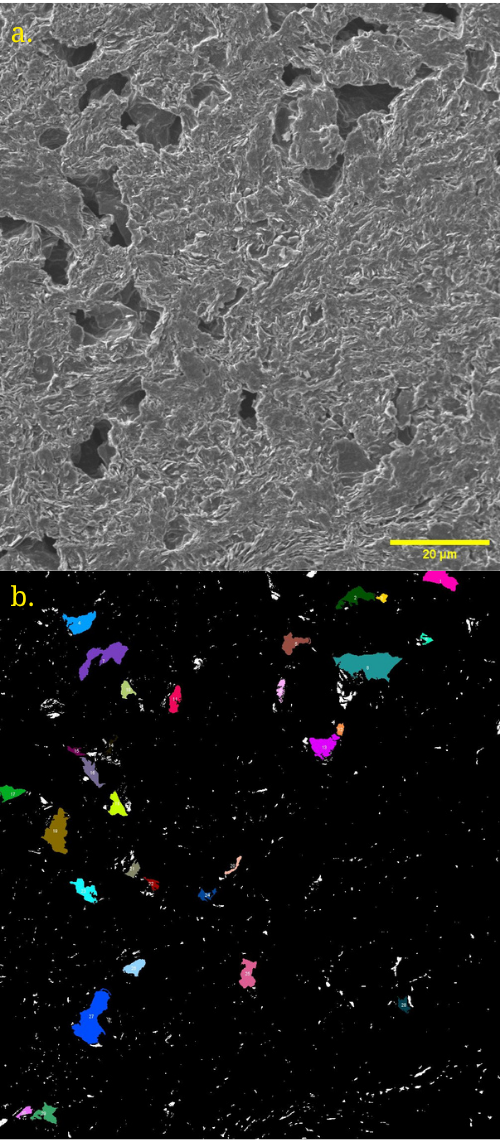
\includegraphics[width=0.9\columnwidth]{./Media/C1-ig430f fused cropped 8 bit one color threshed subsample 2um areathresh}
    \caption{Draft: IG-43F subsample a. Raw and b. After intensity and pore diameter thresholding}
    \label{fig:C1-ig430f fused cropped 8 bit one color threshed subsample 2um areathresh}
\end{figure}

\subsection{Helium (He) Pycnometry}

Helium pycnometry measures the volume of solids via gas displacement, applying
Boyle's Law for multiple states  from which density can be derived for a known
mass \ref{eq:boylestates}. 

\begin{equation} \label{eq:boylestates}
  \mathrm{P}_{1}\,\mathrm{V}_{1} \;=\; \mathrm{P}_{2}\,\mathrm{V}_{2}.
\end{equation}

The dataset containing Skeletal density measurements, and calculations of Closed
Pore Volume (CPV), Open Pore Volume (OPV), and Specific Pore Volume (SPV)
generated by Jones et al. was used \citep{Jones2018}. This dataset represents
helium pycnometry measurements performed on IG-110 and IG-430 sampled from the same block as those
samples which underwent SEM imaging in this work.

A Pycnomatic ATC pycnometer (Thermo Fisher Scientific, Italy) was used to
generate this dataset. Measurements were performed at a temperature of 20.00 ±
0.01\textdegree{}C, for ten replicates per sample, calculating the arithmetic
mean. 

Solid phase volume $V_{\mathrm{SOLID}}$ was calculated assuming a theoretical
density of 2.26 g cm$^{-3}$ for an idealised graphite crystal. 

\subsection{Mercury (Hg) Intrusion Porosimetry}
Mercury intrusion porosimetry operates on the principle that the pressure at
which a non-wetting fluid intrudes a pore is inversely proportional to the
diameter of that pore.

\todo{I mean really it is about connectivity right? But anyhow I might just
leave it as is.}

The exact physical relationship between diameter and applied pressure is
governed by the Laplace Equation (Eq. ~\ref{eq:washburn})
	
	\begin{equation} \label{eq:washburn}
		d = \frac{-4\gamma \cos \theta}{P}
	\end{equation}

	\begin{itemize}
		\item $d$ (m): Pore diameter
		\item $\gamma$ (N/m): Surface tension of the fluid
		\item $\theta$ (degrees): Contact angle of the fluid with the surface
		\item $P$ (Pa): Pressure
	\end{itemize}

140$^{\circ}$ and 130$^{\circ}$ were the values assumed for advancing and
receding contact angles respectively. 0.480 N m$^{-1}$ was taken for the surface
tension of mercury \citep{VANBRAKEL19811}.  

In this work, the dataset generated by Jones et al. \citep{Jones2018} was used,
representing mercury intrusion porosimetry performed on IG-110 and IG-430
sampled from the same block as those samples which underwent SEM imaging in this work.

\subsection{Nitrogen (N$_2$) Adsorption}
Low-pressure gas adsorption isotherms were obtained using a BELSORP-max (MicrotracBEL, Japan)
volumetric gas adsorption instrument.

The dataset generated by Jones \textit{et al}. \citep{Jones2018} was used in
this work, representing nitrogen adsorption measurements performed on IG-110 and
IG-430 sampled from the same block as those samples which underwent SEM imaging
in this work.

\section{Modelling}

PoreXpert is a quasi-Bayesian modelling software which proceeds inversely from
effect (the percolation) to cause (the void network). The software constructs an
8-dimensional parameter space, composed of 5 numerical parameters which
represent the physical characteristics of the pore network, and 3 constraining
Boolean parameters. A Boltzmann-annealed amoeboid simplex searches over this
parameter space to find the set of parameters that produces a percolation curve
minimally different from the intrusion curve derived from Hg porosimetry and
N$_2$/Kr adsorption. The intrusion curve is formed of experimental output from
both methods as mercury porosimetery cannot reach sufficient pressure to probe
the smallest voids of interest, and therefore, the percolation characteristic is
extended to smaller void sizes by Grand-Canonical Monte-Carlo interpretation of
N$_2$ adsorption. The output is a simulated pore network with the matching
porosity and percolation properties, on which simulations such as pore-fluid
permeability and tortuosity can be performed (Figure \ref{fig:PX3dnetwork}
\citep{MatthewsPoreXpert2025}).

During modelling, the approximation type reflecting the depth of SEM analysis
into the porous structure is selected by the user (Figure
\ref{fig:bradapproximationtypesv2.png}, \citep{MatthewsPoreXpert2025}).
Approximation Type 2 \textit{Surface connected throats and the visible volumes
of connected pores} was determined to be the optimal approximation for the
channel porosity dataset, following examination of the micrographs.

\begin{figure}
  \centering
  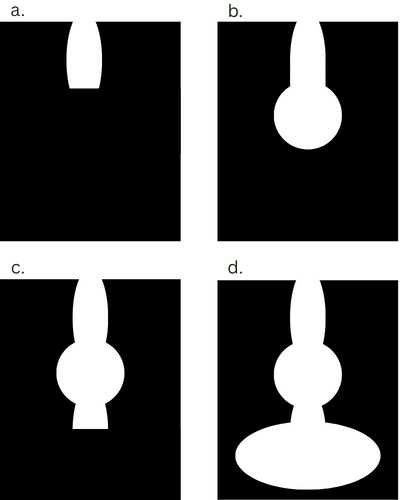
\includegraphics[width=0.9\columnwidth]{./Media/bradapproximationtypesv2.png}
  \caption{Representation of approximation types 1–4. White regions indicate
   porosity visible to the SEM, while black represents bulk.
    (a) Surface-connected throats only. (b) Surface-connected throats along
     with the visible volumes of connected pores. (c) Surface-connected throats,
      visible volumes of connected pores, and any throats located beneath them.
      (d) All vertically aligned features in the top layer, including both
       surface-connected and unconnected elements.}
  \label{fig:pxapproxtypes}
\end{figure}

  Channel porosity (\%), minimum, and maximum pore diameter were input into the
  modelling software. The implementation of a minimum and maximum pore diameter
  enables the  model  to adjust the extent of the PSD which the channel porosity
  estimates. For the initial test sample IG-110B, the simulated intrusion curve
  was optimised to a 1.91\% deviation from the experimental curve.

  (Figure ~\ref{fig:PXfittinggraph})
\begin{figure}
    \centering
    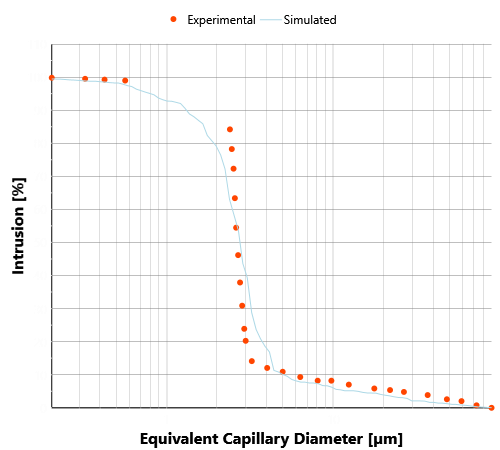
\includegraphics[width=0.9\columnwidth]{./Media/Fit to percolation curve.png}
    \caption{Comparison of the simulated intrusion curve with the experimental data. 
             Orange dots represent experimental data points, while the blue line 
             corresponds to the simulated percolation curve generated from the 
             pore network model.}
    \label{fig:PXfittinggraph}
\end{figure}


      \begin{figure}
        \centering
        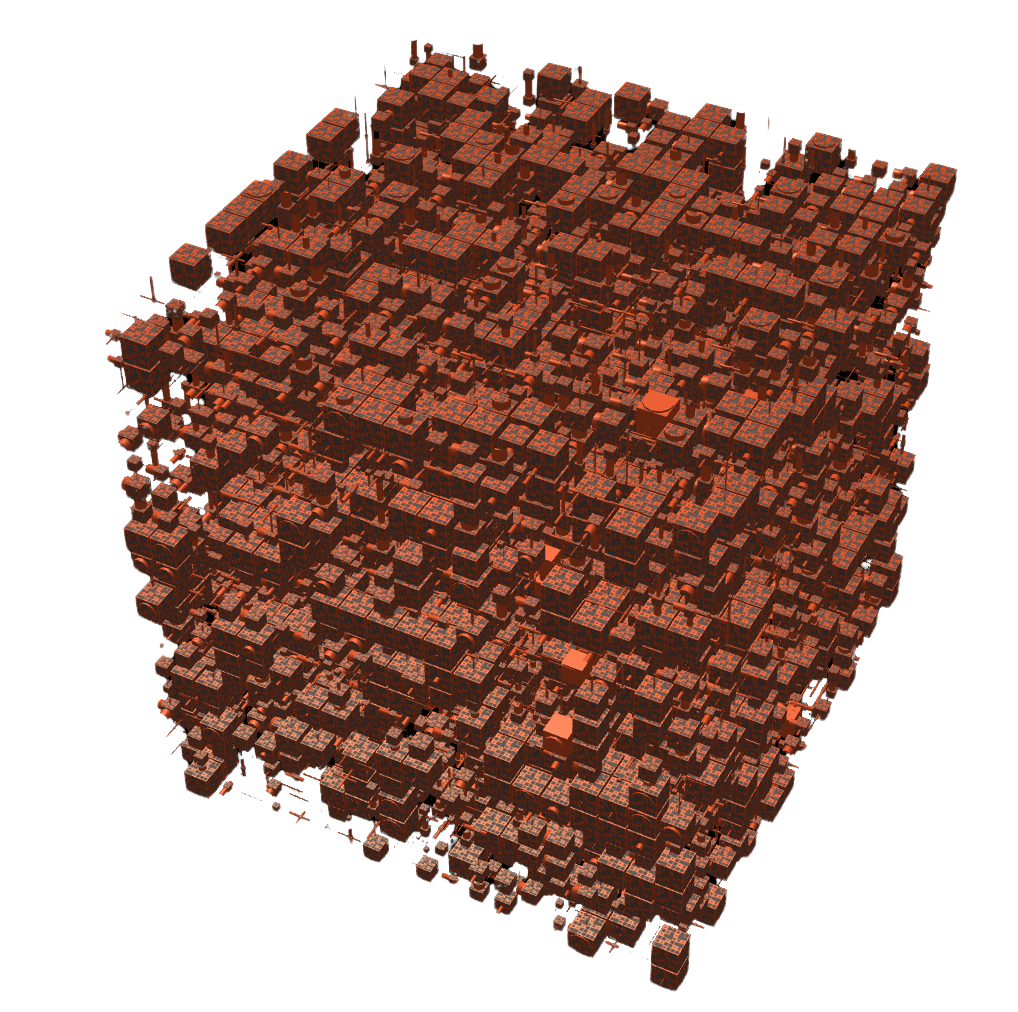
\includegraphics[width=0.9\columnwidth]{./Media/unit cell no bg.png}
        \caption{Pore network resulting from the integration of channel porosity
        and experimental data by the workflows above. 1.91\% distance between
        simulated and experimental curves, following the application of
        Approximation Type 2 (Figure ~\ref{fig:pxapproxtypes}). Channel Porosity
        estimation was averaged over the top 9 layers of a unit cell 20x20x20.
        The result of one generation of stochastic number generation.}
        \label{fig:PX3dnetwork}
    \end{figure}

    Initial modelling outputs were congruent with manufacturer data as
    exemplified for IG-110 Sample B, with an estimated open porosity of 20\%, as
    compared to the 19.62\% figure for the open porosity of IG-110, for Toyo
    Tanso Ltd\texttrademark (Table ~\ref{tab:materialstable}).
    
    The weak correlation (r\(^2\) = 0.32) between open porosity estimate and
    distance between simulated and experimental percolation characteristic
    indicates that averaging over all stochastic generations is a valid measure
    of this method's estimate of open porosity. 

\section{Results}

\begin{table}
  \centering
  \caption{Pore Size Distribution (PSD) and summary characteristics for IG-110 and IG-430 samples.}
  \label{tab:PSDtable}
  \resizebox{\columnwidth}{!}{%
    \begin{tabular}{c c c c}
      \hline
      Sample & n / pores & Total Area / $\mu$m$^2$ & Channel Porosity / \% \\
      \hline
      IG-110 B & 8,684  & 41,091 & 3.14 \\
      IG-110 C & 7,075  & 49,755 & 3.27 \\
      IG-110 F & 8,296  & 50,735 & 3.38 \\
      IG-430 B & 6,848  & 32,983 & 2.30 \\
      IG-430 C & 13,026 & 49,534 & 2.94 \\
      IG-430 F & 6,819  & 56,794 & 3.66 \\
      \hline
    \end{tabular}%
  }
\end{table}

The completed workflow of SEM imaging and computational composite analysis
yielded estimates of channel porosity for both graphite grades (Table
~\ref{tab:PSDtable}). IG-110 samples exhibited channel porosity values ranging
from 3.14-3.38\%, while channel porosity for IG-430 samples ranged from
2.30-3.66\%

\begin{figure}
    \centering
    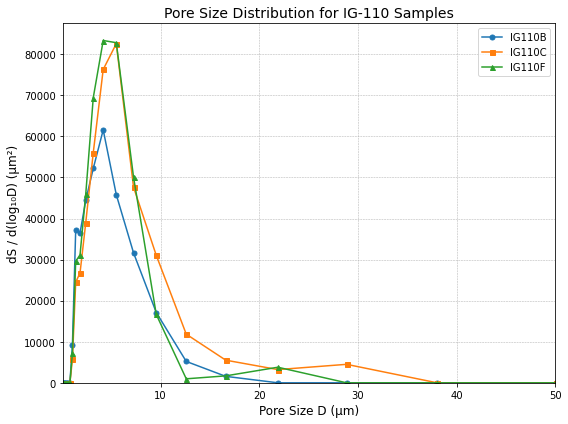
\includegraphics[width=0.9\columnwidth]{./Media/IG110 ds LogD .png}
    \caption{DRAFT: I want to recheck my code on these distributions}
    \label{fig:IG110LogPSDs}
\end{figure}

\begin{figure}
    \centering
    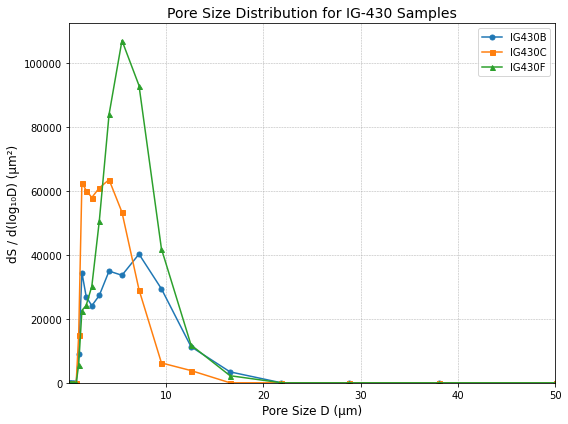
\includegraphics[width=0.9\columnwidth]{./Media/IG430 ds LogD .png}
    \caption{DRAFT: I want to recheck my code on these distributions}
    \label{fig:IG430LogPSDs}
\end{figure}

Area contribution distribution is represented graphically for both graphite
grades (Figure ~\ref{fig:IG110LogPSDs}, ~\ref{fig:IG430LogPSDs}). The area of
each logarithmic bin (spanning 0.1-100 µm on the x-axis) was summed then divided
by the bin width in \(\log_{10}(D)\) to derive \(dS/d(\log_{10}D)\), with the
x-axis then linearised and constrained. y-axis values represent area density in
µm\(^2\) per \(\log_{10}(D)\).

IG-110 and IG-430 exhibit peaks between at 3-7 µm. \citep{huang2021statistical}
found that channel porosity as classified by SEM was 3\% for IG-110, which is
highly congruent with the 3.14-3.38\% range derived in this work.

Interpolation via the adjustment of the intensity threshold to match previous OM
works (i.e., pore contours are classified, as opposed to pore throats) produces
results consistent with previous works. \citep{Kane2011a} derive a channel
porosity of 14.73\% for IG-110, with \citep{Huang2019} deriving 14\% for the
same grade, congruent with the 13-14\% channel porosity derived by this work
following interpolation.

\section{Discussion}

  \subsection{Channel Porosity Overestimation due to connecitivity algo}
  This algorithm is likely to yield at least a slight overestimation of the
average pore size. This is because such an inclusive definition means that two
or more pores, connected by a narrow neck or even simply with adjacent pixels,
would be classified as a single pore. Notably, this would not change the final
channel porosity (\%), nor the modelling, as it utilises only the channel
porosity \%. However, this would result in a rightward shift in the PSD.
Skeleton segmentation is for fine-grade nuclear graphite likely to be a more
accurate approach than a simple connectivity algorithm as used here would be a
key improvement if implemented
\cite{ARREGUIMENA2022112047}

\subsection{Pore Diameter Threshold Discussion}
   Setting the pore diameter  threshold does not imply that no pores exist below
   this limit. Rather, it acknowledges that the confidence in classifying pores
   below the threshold is too low for reliable use. In this work, the
   limitations of any single technique are compensated by the strengths of
   others. during modelling, an interval is selected over which the channel
   porosity determined from SEM imaging can reliably constrain the outputs of
   the inverse modelling process. Thus, no type II errors are introduced in the
   final model due to pore size thresholding, thanks to the combined use of
   alternative techniques and the ability to specify an interval within
   PoreXpert v.3.

   \todo{This part really requires Peter's insight as to the actual functioning of the program}
   \todo{This is not the key issue. The real thing is the accuracy of the pore
   size distribution generated by SEM. For example, the modelling would I think
   be distorted completely by saying that 3\% of the sample surface is made up
   of pores of 1.12-25 µm diameter, when that number may actually represent all
   pores above 1.12 µm, and it is just fragmenting the pores. Being unsure about
   the exact diameter range of pores covered by SEM must surely be making the 
   modelling less accurate, and the pore size distribution more skewed.}

\subsection{Pore Fragmentation and Implications for Modelling}
The application of a maximum pore diameter is a key part of the modelling as
  initial modelling where this was not implemented failed to yield reliable
  results. It is believed that this is due to the impossiblity of the model
  fitting an plausible network on the premise that pores from 1.12 µm diameter
  upwards represent only 3 \% of the sample surface. Imposing an upper threshold
  as the simple max of the pore diameters identified by SEM is an uncomplicated
  initial solution which has more logical implications (i.e., to state that
  between 1.12 and 20um diameter, 3\% of the sample surface is represented by
  porosity). This threshold varied between 13-26 µm in this work, which should
  cover the vast majority of the porosity, particularly given the pore fragmentation
  issue described below.

  Specifically, the use of a simple Moore neighbourhood connectivity, when
  combined with the fact that Erosion and Dilation binary operations were not
  applied, means that pores which the operator identifies as a single pore are
  in more than one case instead defined as two or more pores. Not only this but
  these split pores may not then surpass the pore diameter threshold of 1.12um.
  (e.g., a pore of 10um diameter might be split into 2 pores, 1 of 9um diameter
  and another of 1um diameter, which would be discarded due to the pore diameter
  threshold, reducing the channel porosity \% and shifting rightward the pore
  size distribution).

  The end result is that it is difficult to describe the pore size distribution
  derived from SEM as it currently stands, as completely impenetrable.
  Crucially, the production of reasonable results from the modelling as above
  depends on an accurate constraint of the pore diameter interval (i.e., the
  channel porosity figure of 3\% refers only to porosity between 1.12 and 25um
  diameter) and so not only the SEM-derived pore size distribution but the PX
  modelling which uses it, has at least some reduction in reliability due to the
  pore fragmentation issue. However, this is likely a soluble problem, as
  follows (look at workflow).

    \subsection{Proposed Future Workflow}

  -Just my idea of an improved workflow:
  1. Resin Impregnation
  2. SEM (see if we can go to 2kV)
  3. Otsu Thresholding (We have clear bimodality thanks to Resin impregnation)
  4. Skeleton segmentation (Avizo software needed?)
  5. Apply improved pore diameter thresholds, or maybe do not do any at all as no longer needed? At least lowered.
  6. Modelling

    \subsection{Proposed Improved Sample Preparation}

  \todo{Could talk here about how we wanted to do resin impeg like Kane et al, but
  did not have the chance, and explain this might introduce issues, also we
  could talk about how this is quite rough, and that this kind of sample
  preparation (i.e. no vibratory polishing, no resin impregnation) is not ideal
  and may have introduced both artefacts and noise. Additionally, sonication may
  have damaged the pore structure}


\section{Supplementary Information}

One advantage of this method is the avoidance of error propagation by
consecutive registration steps, as simply placing micrograph A relative to
micrograph B, and then micrograph B relative to micrograph C, would result in
accumulation of errors. This method builds a graph whose nodes are the
micrographs, and edges are the measured pairwise shifts between the micrographs.
It then finds the set of micrograph positions that minimise the total squared
registration error across the entire graph, a form of globally optimised
registration \citep{Preibisch2009}.

This stitching method also allows sub-pixel accuracy, which is crucial for
accurate pore measurement. For any two micrographs \(A\) and \(B\), which are
shifted relative to each other (i.e., micrograph \(B\) is shifted two pixels up
and 10 pixels left of micrograph \(A\)) then their Fourier transforms would
have the same magnitude but different phases. A normalized cross-power spectrum
isolates the phase difference, and the Inverse Fourier transform
yields a correlation map with peaks indicating possible translations between the
micrographs. The complexity of real images and the periodicity of the Fourier
transform means that the correlation map is not a single peak, but rather a set
of peaks, each representing a possible translation. This method therefore
selects the \(n\) highest local maxima and finds the peak with the best
correlation, which it defines as the true translation between the two
micrographs \citep{Preibisch2009}. Finally, sub-pixel accuracy in that shift is
achieved by applying a parabolic interpolation around the selected peak to
refine the translation estimate.

Additionally, a non-linear intensity blending function eliminates the visible
seams between micrographs, which can occur even when the micrographs are
perfectly aligned due to shading variations. This blending assigns a weight to
each pixel in a tile, working as a function of the distance from the tile edge,
with a tunable parameter controlling this weighting function. In non-overlapping
regions, the centre of the micrograph, the weight is essentially 1, so the
original pixel value is preserved exactly. In overlapping regions, intensities
are a convex combination of the original values. Crucially, because the weights
sum to 1 everywhere, blended intensity is simply a weighted average of the
original intensities. Thus, the final composite micrograph is still a valid
representation of the original micrographs, but the seams have been removed.
\citep{Preibisch2009}  The removal of the visible seams between micrographs did
increase confidence that in the following steps, the subsample used to determine
the intensity threshold was representative of the full composite micrograph.
\clearpage

\bibliography{bibliography}
\end{document}